% Created by tikzDevice version 0.12.3.1 on 2022-06-13 20:17:43
% !TEX encoding = UTF-8 Unicode
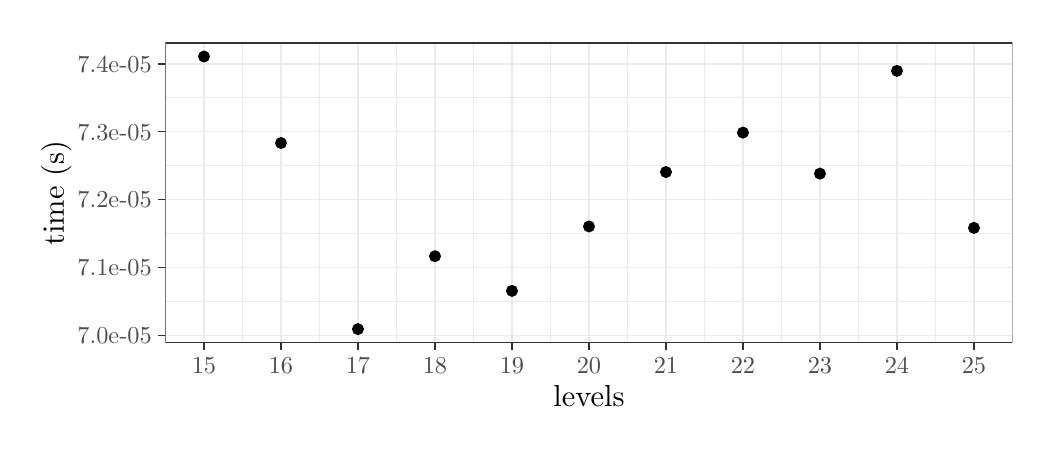
\begin{tikzpicture}[x=1pt,y=1pt]
\definecolor{fillColor}{RGB}{255,255,255}
\path[use as bounding box,fill=fillColor,fill opacity=0.00] (0,0) rectangle (361.35,144.54);
\begin{scope}
\path[clip] (  0.00,  0.00) rectangle (361.35,144.54);
\definecolor{drawColor}{RGB}{255,255,255}
\definecolor{fillColor}{RGB}{255,255,255}

\path[draw=drawColor,line width= 0.6pt,line join=round,line cap=round,fill=fillColor] (  0.00,  0.00) rectangle (361.35,144.54);
\end{scope}
\begin{scope}
\path[clip] ( 49.80, 30.69) rectangle (355.85,139.04);
\definecolor{fillColor}{RGB}{255,255,255}

\path[fill=fillColor] ( 49.80, 30.69) rectangle (355.85,139.04);
\definecolor{drawColor}{gray}{0.92}

\path[draw=drawColor,line width= 0.3pt,line join=round] ( 49.80, 45.59) --
	(355.85, 45.59);

\path[draw=drawColor,line width= 0.3pt,line join=round] ( 49.80, 70.14) --
	(355.85, 70.14);

\path[draw=drawColor,line width= 0.3pt,line join=round] ( 49.80, 94.69) --
	(355.85, 94.69);

\path[draw=drawColor,line width= 0.3pt,line join=round] ( 49.80,119.24) --
	(355.85,119.24);

\path[draw=drawColor,line width= 0.3pt,line join=round] ( 49.80, 30.69) --
	( 49.80,139.04);

\path[draw=drawColor,line width= 0.3pt,line join=round] ( 77.62, 30.69) --
	( 77.62,139.04);

\path[draw=drawColor,line width= 0.3pt,line join=round] (105.44, 30.69) --
	(105.44,139.04);

\path[draw=drawColor,line width= 0.3pt,line join=round] (133.27, 30.69) --
	(133.27,139.04);

\path[draw=drawColor,line width= 0.3pt,line join=round] (161.09, 30.69) --
	(161.09,139.04);

\path[draw=drawColor,line width= 0.3pt,line join=round] (188.91, 30.69) --
	(188.91,139.04);

\path[draw=drawColor,line width= 0.3pt,line join=round] (216.73, 30.69) --
	(216.73,139.04);

\path[draw=drawColor,line width= 0.3pt,line join=round] (244.56, 30.69) --
	(244.56,139.04);

\path[draw=drawColor,line width= 0.3pt,line join=round] (272.38, 30.69) --
	(272.38,139.04);

\path[draw=drawColor,line width= 0.3pt,line join=round] (300.20, 30.69) --
	(300.20,139.04);

\path[draw=drawColor,line width= 0.3pt,line join=round] (328.03, 30.69) --
	(328.03,139.04);

\path[draw=drawColor,line width= 0.3pt,line join=round] (355.85, 30.69) --
	(355.85,139.04);

\path[draw=drawColor,line width= 0.6pt,line join=round] ( 49.80, 33.32) --
	(355.85, 33.32);

\path[draw=drawColor,line width= 0.6pt,line join=round] ( 49.80, 57.87) --
	(355.85, 57.87);

\path[draw=drawColor,line width= 0.6pt,line join=round] ( 49.80, 82.42) --
	(355.85, 82.42);

\path[draw=drawColor,line width= 0.6pt,line join=round] ( 49.80,106.96) --
	(355.85,106.96);

\path[draw=drawColor,line width= 0.6pt,line join=round] ( 49.80,131.51) --
	(355.85,131.51);

\path[draw=drawColor,line width= 0.6pt,line join=round] ( 63.71, 30.69) --
	( 63.71,139.04);

\path[draw=drawColor,line width= 0.6pt,line join=round] ( 91.53, 30.69) --
	( 91.53,139.04);

\path[draw=drawColor,line width= 0.6pt,line join=round] (119.35, 30.69) --
	(119.35,139.04);

\path[draw=drawColor,line width= 0.6pt,line join=round] (147.18, 30.69) --
	(147.18,139.04);

\path[draw=drawColor,line width= 0.6pt,line join=round] (175.00, 30.69) --
	(175.00,139.04);

\path[draw=drawColor,line width= 0.6pt,line join=round] (202.82, 30.69) --
	(202.82,139.04);

\path[draw=drawColor,line width= 0.6pt,line join=round] (230.65, 30.69) --
	(230.65,139.04);

\path[draw=drawColor,line width= 0.6pt,line join=round] (258.47, 30.69) --
	(258.47,139.04);

\path[draw=drawColor,line width= 0.6pt,line join=round] (286.29, 30.69) --
	(286.29,139.04);

\path[draw=drawColor,line width= 0.6pt,line join=round] (314.12, 30.69) --
	(314.12,139.04);

\path[draw=drawColor,line width= 0.6pt,line join=round] (341.94, 30.69) --
	(341.94,139.04);
\definecolor{drawColor}{RGB}{0,0,0}
\definecolor{fillColor}{RGB}{0,0,0}

\path[draw=drawColor,line width= 0.4pt,line join=round,line cap=round,fill=fillColor] ( 63.71,134.11) circle (  1.96);

\path[draw=drawColor,line width= 0.4pt,line join=round,line cap=round,fill=fillColor] ( 91.53,102.87) circle (  1.96);

\path[draw=drawColor,line width= 0.4pt,line join=round,line cap=round,fill=fillColor] (119.35, 35.61) circle (  1.96);

\path[draw=drawColor,line width= 0.4pt,line join=round,line cap=round,fill=fillColor] (147.18, 61.96) circle (  1.96);

\path[draw=drawColor,line width= 0.4pt,line join=round,line cap=round,fill=fillColor] (175.00, 49.43) circle (  1.96);

\path[draw=drawColor,line width= 0.4pt,line join=round,line cap=round,fill=fillColor] (202.82, 72.71) circle (  1.96);

\path[draw=drawColor,line width= 0.4pt,line join=round,line cap=round,fill=fillColor] (230.65, 92.37) circle (  1.96);

\path[draw=drawColor,line width= 0.4pt,line join=round,line cap=round,fill=fillColor] (258.47,106.62) circle (  1.96);

\path[draw=drawColor,line width= 0.4pt,line join=round,line cap=round,fill=fillColor] (286.29, 91.80) circle (  1.96);

\path[draw=drawColor,line width= 0.4pt,line join=round,line cap=round,fill=fillColor] (314.12,128.93) circle (  1.96);

\path[draw=drawColor,line width= 0.4pt,line join=round,line cap=round,fill=fillColor] (341.94, 72.19) circle (  1.96);
\definecolor{drawColor}{gray}{0.20}

\path[draw=drawColor,line width= 0.6pt,line join=round,line cap=round] ( 49.80, 30.69) rectangle (355.85,139.04);
\end{scope}
\begin{scope}
\path[clip] (  0.00,  0.00) rectangle (361.35,144.54);
\definecolor{drawColor}{gray}{0.30}

\node[text=drawColor,anchor=base east,inner sep=0pt, outer sep=0pt, scale=  0.88] at ( 44.85, 30.29) {7.0e-05};

\node[text=drawColor,anchor=base east,inner sep=0pt, outer sep=0pt, scale=  0.88] at ( 44.85, 54.84) {7.1e-05};

\node[text=drawColor,anchor=base east,inner sep=0pt, outer sep=0pt, scale=  0.88] at ( 44.85, 79.39) {7.2e-05};

\node[text=drawColor,anchor=base east,inner sep=0pt, outer sep=0pt, scale=  0.88] at ( 44.85,103.93) {7.3e-05};

\node[text=drawColor,anchor=base east,inner sep=0pt, outer sep=0pt, scale=  0.88] at ( 44.85,128.48) {7.4e-05};
\end{scope}
\begin{scope}
\path[clip] (  0.00,  0.00) rectangle (361.35,144.54);
\definecolor{drawColor}{gray}{0.20}

\path[draw=drawColor,line width= 0.6pt,line join=round] ( 47.05, 33.32) --
	( 49.80, 33.32);

\path[draw=drawColor,line width= 0.6pt,line join=round] ( 47.05, 57.87) --
	( 49.80, 57.87);

\path[draw=drawColor,line width= 0.6pt,line join=round] ( 47.05, 82.42) --
	( 49.80, 82.42);

\path[draw=drawColor,line width= 0.6pt,line join=round] ( 47.05,106.96) --
	( 49.80,106.96);

\path[draw=drawColor,line width= 0.6pt,line join=round] ( 47.05,131.51) --
	( 49.80,131.51);
\end{scope}
\begin{scope}
\path[clip] (  0.00,  0.00) rectangle (361.35,144.54);
\definecolor{drawColor}{gray}{0.20}

\path[draw=drawColor,line width= 0.6pt,line join=round] ( 63.71, 27.94) --
	( 63.71, 30.69);

\path[draw=drawColor,line width= 0.6pt,line join=round] ( 91.53, 27.94) --
	( 91.53, 30.69);

\path[draw=drawColor,line width= 0.6pt,line join=round] (119.35, 27.94) --
	(119.35, 30.69);

\path[draw=drawColor,line width= 0.6pt,line join=round] (147.18, 27.94) --
	(147.18, 30.69);

\path[draw=drawColor,line width= 0.6pt,line join=round] (175.00, 27.94) --
	(175.00, 30.69);

\path[draw=drawColor,line width= 0.6pt,line join=round] (202.82, 27.94) --
	(202.82, 30.69);

\path[draw=drawColor,line width= 0.6pt,line join=round] (230.65, 27.94) --
	(230.65, 30.69);

\path[draw=drawColor,line width= 0.6pt,line join=round] (258.47, 27.94) --
	(258.47, 30.69);

\path[draw=drawColor,line width= 0.6pt,line join=round] (286.29, 27.94) --
	(286.29, 30.69);

\path[draw=drawColor,line width= 0.6pt,line join=round] (314.12, 27.94) --
	(314.12, 30.69);

\path[draw=drawColor,line width= 0.6pt,line join=round] (341.94, 27.94) --
	(341.94, 30.69);
\end{scope}
\begin{scope}
\path[clip] (  0.00,  0.00) rectangle (361.35,144.54);
\definecolor{drawColor}{gray}{0.30}

\node[text=drawColor,anchor=base,inner sep=0pt, outer sep=0pt, scale=  0.88] at ( 63.71, 19.68) {15};

\node[text=drawColor,anchor=base,inner sep=0pt, outer sep=0pt, scale=  0.88] at ( 91.53, 19.68) {16};

\node[text=drawColor,anchor=base,inner sep=0pt, outer sep=0pt, scale=  0.88] at (119.35, 19.68) {17};

\node[text=drawColor,anchor=base,inner sep=0pt, outer sep=0pt, scale=  0.88] at (147.18, 19.68) {18};

\node[text=drawColor,anchor=base,inner sep=0pt, outer sep=0pt, scale=  0.88] at (175.00, 19.68) {19};

\node[text=drawColor,anchor=base,inner sep=0pt, outer sep=0pt, scale=  0.88] at (202.82, 19.68) {20};

\node[text=drawColor,anchor=base,inner sep=0pt, outer sep=0pt, scale=  0.88] at (230.65, 19.68) {21};

\node[text=drawColor,anchor=base,inner sep=0pt, outer sep=0pt, scale=  0.88] at (258.47, 19.68) {22};

\node[text=drawColor,anchor=base,inner sep=0pt, outer sep=0pt, scale=  0.88] at (286.29, 19.68) {23};

\node[text=drawColor,anchor=base,inner sep=0pt, outer sep=0pt, scale=  0.88] at (314.12, 19.68) {24};

\node[text=drawColor,anchor=base,inner sep=0pt, outer sep=0pt, scale=  0.88] at (341.94, 19.68) {25};
\end{scope}
\begin{scope}
\path[clip] (  0.00,  0.00) rectangle (361.35,144.54);
\definecolor{drawColor}{RGB}{0,0,0}

\node[text=drawColor,anchor=base,inner sep=0pt, outer sep=0pt, scale=  1.10] at (202.82,  7.64) {levels};
\end{scope}
\begin{scope}
\path[clip] (  0.00,  0.00) rectangle (361.35,144.54);
\definecolor{drawColor}{RGB}{0,0,0}

\node[text=drawColor,rotate= 90.00,anchor=base,inner sep=0pt, outer sep=0pt, scale=  1.10] at ( 13.08, 84.86) {time (s)};
\end{scope}
\end{tikzpicture}
